\documentclass{article}

\usepackage[margin=0.8in]{geometry}
\usepackage{amsmath, amsfonts}
\usepackage{hyperref}
\usepackage{xcolor}
\usepackage{subcaption}
\usepackage{caption}
\usepackage{graphicx}

\setlength{\parindent}{0pt}

\begin{document}

\begin{center}
    \begin{tabular}{ccc}
        \shortstack{Initial $Q$-values \\ \includegraphics[width=0.35\textwidth]{Figures/q_mb.pdf}} &  \\
        \shortstack{Exploratory replay (sequence) \\ \includegraphics[width=0.35\textwidth]{Figures/replay_explore.pdf}} & \shortstack{Value difference \\ \includegraphics[width=0.35\textwidth]{Figures/replay_explore_diff.pdf}}\\
        \shortstack{Online learning \\ \includegraphics[width=0.35\textwidth]{Figures/online.pdf}} & \shortstack{Value difference \\ 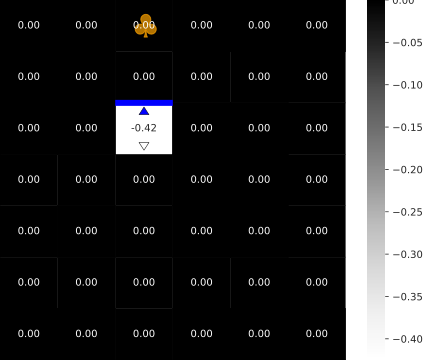
\includegraphics[width=0.35\textwidth]{Figures/online_diff.pdf}} \\
        \shortstack{"Negative" replay (sequence) \\ \includegraphics[width=0.35\textwidth]{Figures/replay_negative.pdf}} & \shortstack{Value difference \\ \includegraphics[width=0.35\textwidth]{Figures/replay_negative_diff.pdf}}
    \end{tabular}
\end{center}

\end{document}
